\lsection{Mapa i orientacja przestrzenna}
    W celach testowych została napisana aplikacja graficzna do sterowani pojazdem, oraz reprezentująca mapę użytkownikowi.
    Na zdjęciu \ref{fig:app} przedstawiono interfejs aplikacji.
    \begin{figure}[!ht]
        \centering
        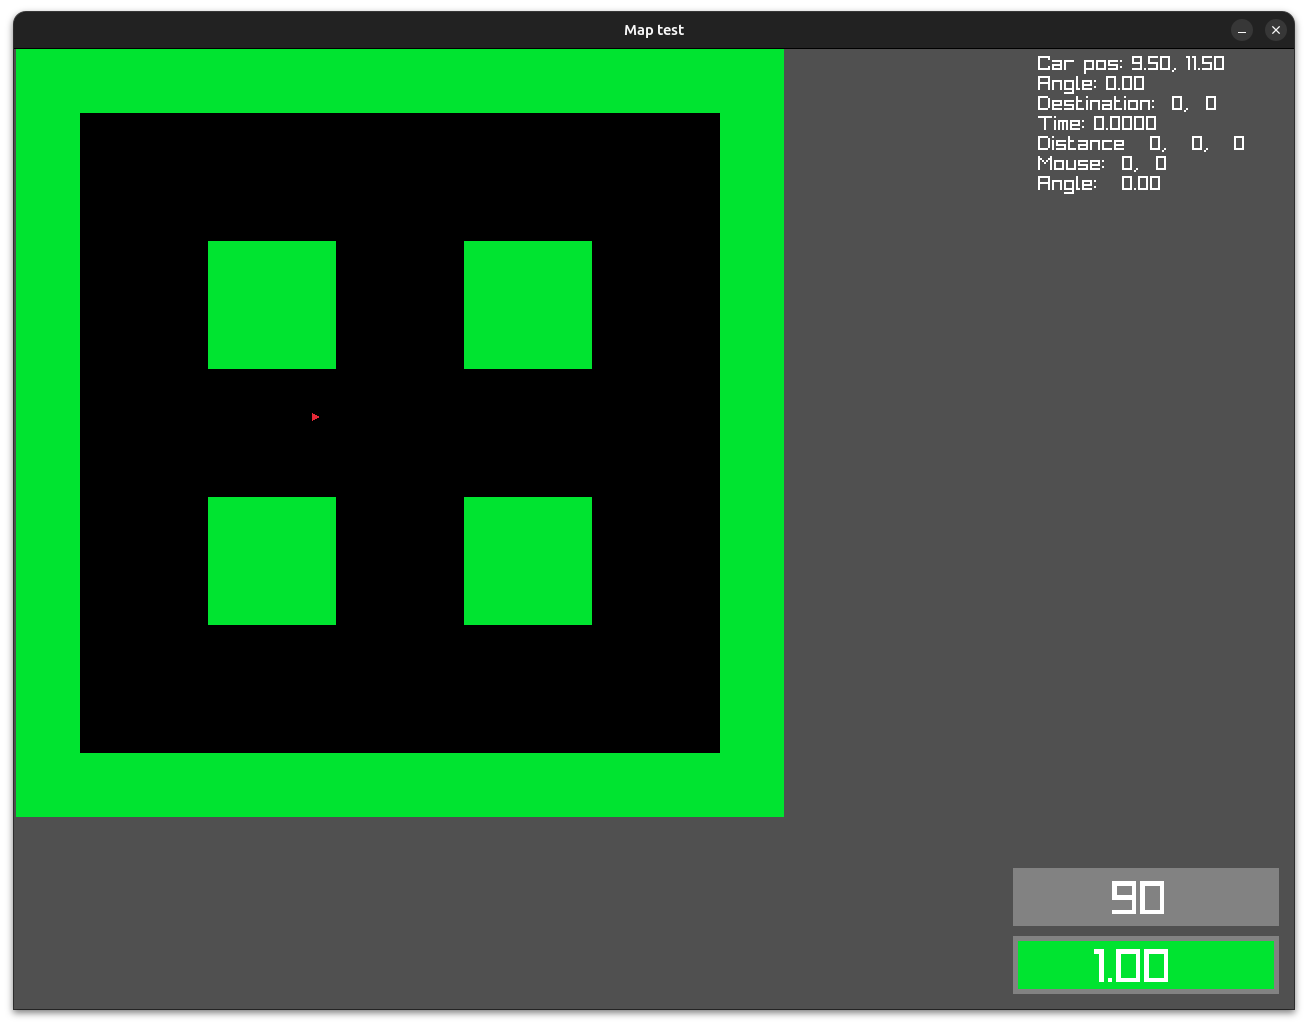
\includegraphics[width = 0.7\textwidth]{PathFinding/App.png}
        \caption{Interfejs aplikacji}
        \label{fig:app}
    \end{figure}
    Interfejs aplikacji składa się z trzech części:
    \begin{enumerate}
        \item Mapa -- reprezentująca aktualnie zbadanego obszar oraz aktualną pozycję pojazdu.
        \item Informacje -- w prawym górnym rogu, wyświetlane są dodatkowe informacje, takie jak aktualna pozycja pojazdu, czy myszy.
        \item Ślizgacze -- w prawym dolnym rogu, znajdują się dwa ślizgacze, górny pozwala precyzyjnie ustawić kąt skrętu kół a dolny pozwala na ustawienie prędkości pojazdu.
    \end{enumerate}

    \subsection{Budowa mapy}
        W założeniu aplikacja ma pozwalać jedynie na wyświetlanie, mapy zbudowanej przez samochód.
        Natomiast wszystkie obliczenia powinny zostać wykonane przez kontroler zarządzający pojazdem.
        Jednak ze względu na duże skomplikowanie opisywanych problemów, w celach testowych, to aplikacja posiada zaimplementowany algorytm do wyszukiwania ścieżek.
        Następnie wyznaczona ścieżka zamieniana jest na proste instrukcje w stylu ,,uruchom oba silniki na 500mm'' czy ,,skręć kołami o $30^\circ$ w lewo''.
        



    \subsection{Wyznaczanie ścieżek}
        Kliknięcie na mapę, pozwala na wybranie punktu docelowego, do które zostanie wyznaczona ścieżka, po której pojazd będzie się poruszał.

        \subsubsection{Algorytm odnajdowania ścieżek}
            Wyznaczanie optymalnej ścieżki, od wielu lat jest bardzo popularnym problemem w informatyce i robotyce.
            Istnieje wiele artykułów, skupiających się na tej tematyce, a także wiele gotowych rozwiązań.
            Najpopularniejszymi algorytmami są:
            \begin{itemize}
                \item algorytm A* (A star),
                \item algorytm Dijkstra,
                \item algorytm Bellmana-Forda.
            \end{itemize}

            Poniżej przedstawione zostaną wyniki pracy \citetitle{AnalizaAlgorytmówŚcieżek} \cite{AnalizaAlgorytmówŚcieżek}
            autorstwa: Beata \citeauthor{AnalizaAlgorytmówŚcieżek}.
            \begin{figure}[!ht]
                \centering
                \figurePlotName
                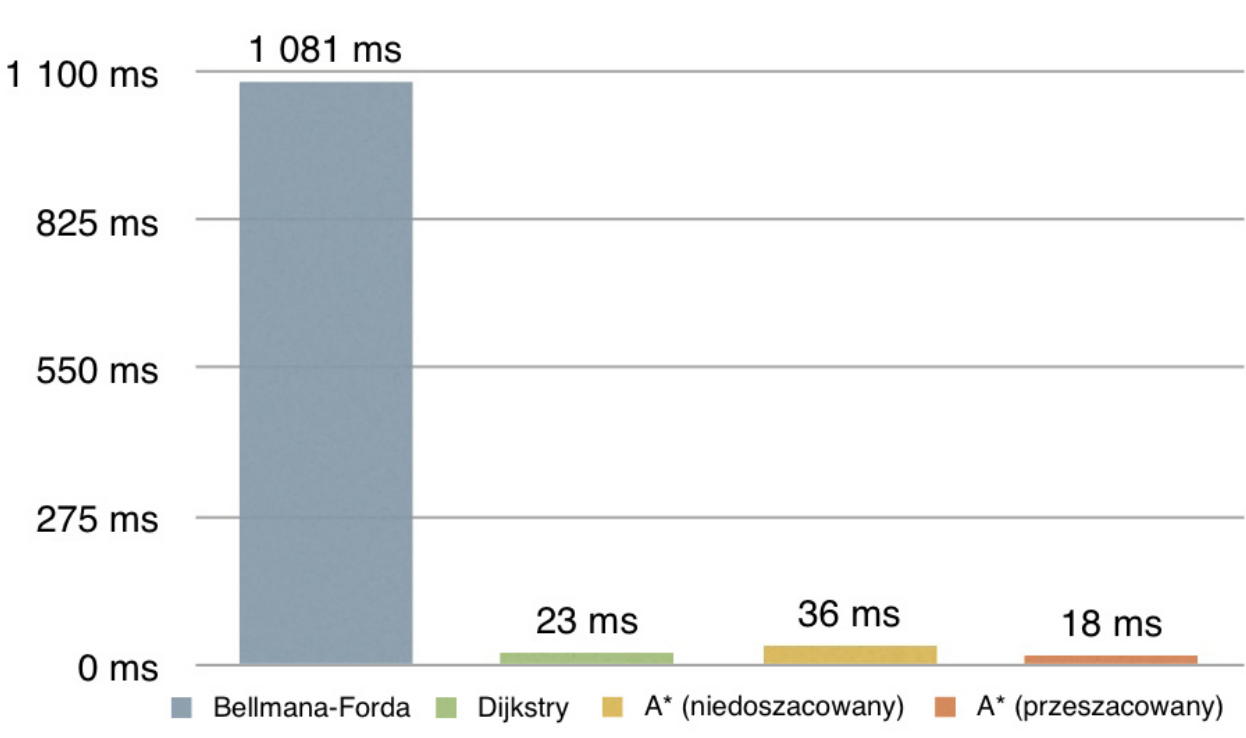
\includegraphics[width=0.7\textwidth]{PathFinding/Wykres_sredni_czas_algorytmu_pathfinding.png}
                \caption{Porównanie średniego czasu wykonania algorytmów}
                Źródło:\cite{AnalizaAlgorytmówŚcieżek} \citetitle{AnalizaAlgorytmówŚcieżek} 
                \label{fig:PathFindingTime}
            \end{figure}
            \begin{figure}[!ht]
                \centering
                \figurePlotName
                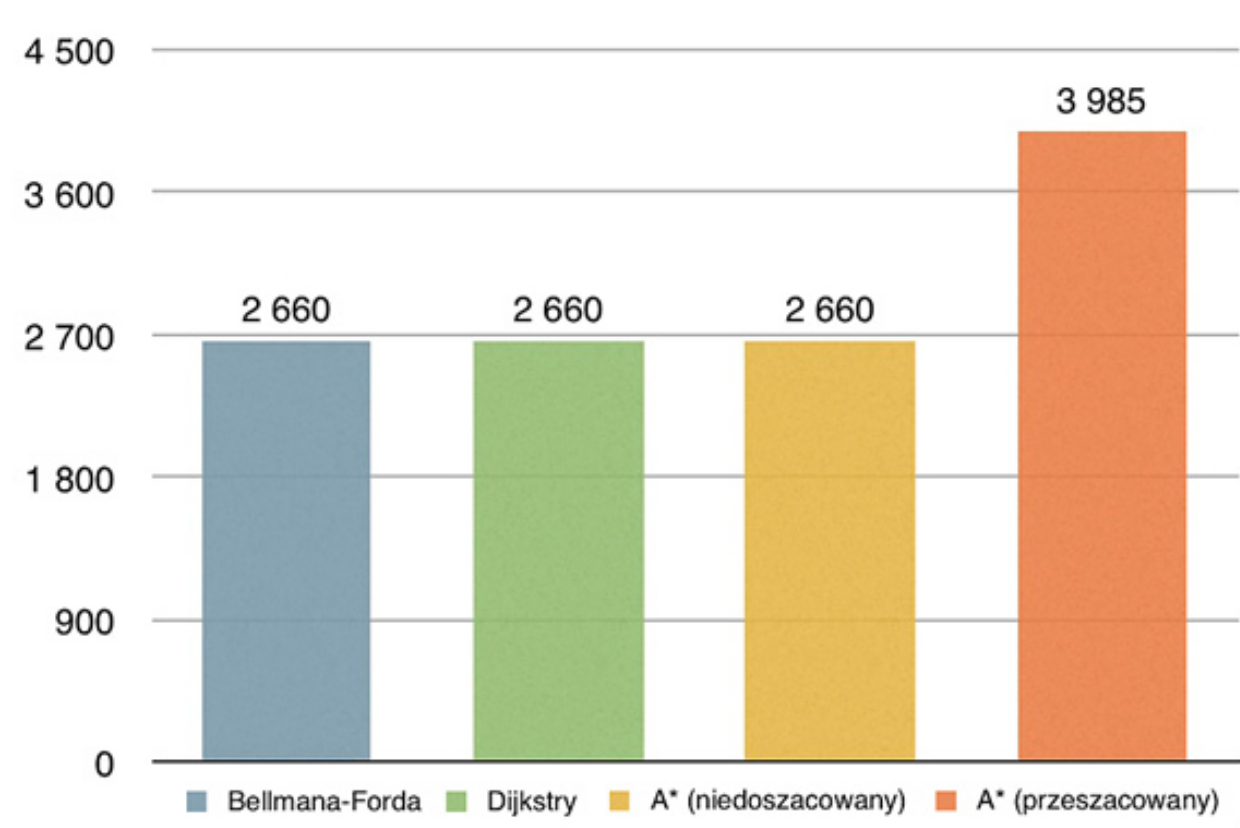
\includegraphics[width=0.7\textwidth]{PathFinding/Wykres_sredni_koszt_algorytmu_pathfinding.png}
                \caption{Porównanie średniego kosztu znalezionych ścieżek}
                Źródło:\cite{AnalizaAlgorytmówŚcieżek} \citetitle{AnalizaAlgorytmówŚcieżek}
                \label{fig:PathFindingCost}
            \end{figure}
            
            Z powyższej pracy wynika, że najlepszym rozwiązaniem jest algorytm Dijkstry.
            Dodatkowym czynnikiem, potwierdzającą powyższe stwierdzenie jest samo skomplikowanie algorytmu.
            Algorytm Dijkstry jest stosunkowo prosty w implementacji, a także posiada niski koszt obliczeniowy.
            Dzięki czemu wydaje się najlepszym rozwiązaniem dla zastosowań w układach embedded.



    
\lsection{Sterowanie pojazdem}
    Sterowanie pojazdem powinno odbywać się w sposób płynny i precyzyjny.
    W poniższym rozdziale zostaną omówione algorytmy, odpowiedzialne za najbardziej podstawowe funkcje poruszania się takie jak: jazda prosto, skręt oraz cofanie.

    \subsection{Jazda przez pewien odcinek}
    \label{subsec:sterowanie_odległość}
        W rozdziale \ref{section:jazda_prosto}, zostały opisane problemy jakie wystąpiły podczas budowy pojazdu. %oraz problemy jakie musiały zostać rozwiązane aby samochód był w stanie jechać prosto.
        Dzięki rozwiązaniu wyżej wymienionych problemów, pojazd był w stanie jechać prosto.
        Jednak dla precyzyjnego sterowania, informacja o tym, że pojazd porusza po linii prostej, jest niewystarczająca.
        Obowiązkowym jest poznanie odległości jaką pokonuje pojazd.

        Wartość odległości jaką pokonuje pojazd od momentu startu, możemy dość dokładnie obliczyć, korzystając ze wzoru \eqref{eq:pulseToDistance}.
        \begin{gather}
            s = \frac{\text{pulse} \cdot 2\pi R}{N}
            \label{eq:pulseToDistance}
        \end{gather}
        gdzie:
        \begin{itemize}
            \item $s$ -- odległość jaką pokonał pojazd,
            \item $\text{pulse}$ -- liczba impulsów z enkodera,
            \item $R$ -- promień koła,
            \item $N$ -- liczba impulsów na obrót koła.
        \end{itemize}

        Wzór ten, można także przekształcić w drugą stronę, aby obliczyć ile impulsów enkodera musi zostać zliczonych, przez procesor aby pojazd pokonał zadaną odległość.
        \begin{gather}
            \text{pulse} = \frac{s \cdot N}{2\pi R}
            \label{eq:distanceToPulse}
        \end{gather}

        Dla zbudowanego modelu, promień koła wynosi $R = 50cm$, a liczba impulsów zgodnie z dokumentacją wynosi $N = 1920$.
        A więc dokładność pomiaru odległości wynosi około:
        \begin{gather}
            \Delta s \approx \pm2.0mm
        \end{gather}


    \subsection{Wyznaczanie zakrętów}
        Wyznaczenie idealnie prostej trasy dla pojazdów nie zawsze jest możliwe.
        W trakcie jazdy, pojazd będzie skręcał wielotonie, w każdym możliwym kierunku.
        Dlatego niezwykle ważne jest, aby zachować maksymalną precyzję podczas skręcania.

        Aby wyznaczyć w jaki sposób nasz samochód powinien skręcić, musi wyznaczyć kilka podstawowych parametrów.
        A są to:
        \begin{itemize}
            \item długość łuku,
            \item promień skrętu,
            \item kąt skrętu kół.
        \end{itemize}
        Na tej podstawie, możemy stworzyć zależność, która pozwoli na napisanie instrukcji dla samochodu, w jaki sposób ma się poruszać.
        \begin{gather}
            s = 2\pi (r(\gamma) + \Delta r) \cdot \frac{\alpha}{360}
            \label{eq:turning_arc}
            \\
            \alpha = \frac{2\pi (r(\gamma + \Delta r))}{s \cdot 360}
        \end{gather}
        gdzie:
        \begin{itemize}
            \item $s$ -- długość łuku,
            \item $r(\gamma)$ -- promień skrętu wyznaczany zgodnie z równaniem \eqref{eq:turning_radius},
            \item $\Delta r$ -- odległość między kołami,
            \item $\alpha$ -- oczekiwany kąt skrętu.
        \end{itemize}

        Dzięki rozważaniom z rozdziału \ref{subsec:sterowanie_odległość}, oraz równaniu \eqref{eq:turning_arc} i \eqref{eq:turning_radius}.
        Możemy stworzyć prostą logikę odpowiedzialną za skręcanie pojazdu.


        \subsubsection{Minimalny promień skrętu}
        \label{subsubsec:minamalny_promien}
            Wyznaczenie promienia skrętu jest 
            \begin{gather}
                2\pi (r + \Delta r) \cdot \frac{\Delta \alpha}{360^\circ} = s\\
                r + \Delta r = \frac{s}{2\pi \cdot \frac{\Delta \alpha}{360^\circ}}
            \end{gather}
            gdzie:
            \begin{itemize}
                \item $r + \Delta r$ -- promień skrętu zewnętrznego koła,
                \item $\Delta \alpha$ -- zakreślony kąt,
                \item $s$ -- długość łuku.
            \end{itemize}

            Zbudowany pojazd, ma możliwość jazdy przez zadaną odległość. 
            Odległość pokonana przez samochód jest dość precyzyjne mierzona przez enkodery,
            a pomiary odległości za pomocą czujników ToF pozwalają na zaufanie dla wartości zadanej.

            Dzięki rozważaniom z rozdziału \ref{subsubsec:dyferencjal} udało się uzyskać powtarzalności pomiarów zakreślonego kąta.
            I tak przykładowo, dla ustawionego maksymalnego kąta skrętu kół $\gamma = 90 \pm 30^\circ$ oraz długości łuku $s = 500mm$, wartość zakreślony kąt wynosił około $\Delta \alpha = \left(60.0 \pm 3.0\right)^\circ$.
            Wartość promienia skrętu wynosiła około:
            \begin{gather}
                r = \frac{500mm}{2\pi \cdot \frac{60 \pm 3.0}{360}} - 125mm \approx (340 \pm 20)mm
            \end{gather}

            Przedstawiony minimalny promień skrętu, możemy oczywiści porównać zgodnie z równaniem \eqref{eq:turning_radius}.
            Po podstawieniu wyżej wymienionych wartości, otrzymujemy:
            \begin{gather}
                r(\gamma = 90 \pm 30^\circ) = \left|\frac{155}{\tan(\pm 30^\circ)}\right| \approx 270mm
            \end{gather}

            Teoretyczny minimalny promień skręty, wychodzący z obliczeń, jest znacząco mniejszy od zmierzonego minimalnego promienia skrętu.
            Wynika to z nie idealności konstrukcji, oraz zastosowania ,,względnie słabej jakości" serwomechanizmu.
            Pojazd nie jest w stanie skręcić kołami jednakowo w obie strony, co wymusiło ustawienie wartości offsetu, przesuwającej wartość kąta skrętu.
            Dla pojazdu testowego, wartość offsetu wynosiła $-6^\circ$. 
            Co ogranicza maksymalny zakres skrętu do $\pm 23^\circ$.
            \begin{gather}
                r(\gamma = 90 \pm 23^\circ) = \left|\frac{155}{\tan(\pm 23^\circ)}\right| \approx 350mm
            \end{gather}

